\documentclass[11pt]{article}
\usepackage{verbatim}
\usepackage[hyphens]{url}
\usepackage{cite}
\usepackage{enumerate}
\setlength{\parindent}{0pt}
\setlength{\parskip}{10pt plus 6pt minus 4pt}
\usepackage{amsmath}
\usepackage{graphicx}
\usepackage[colorinlistoftodos]{todonotes}
\usepackage[colorlinks=true, allcolors=blue]{hyperref}
\title{ Lung Cancer Detection Project \\ Advanced Machine Learning}
\author{}
\date{}


\begin{document}
\maketitle

\section{Team Members}

\begin{itemize}
\item Connor Ameres
\item Andre Duarte
\item Nicholas Levitt
\item Juan Pablo Oberhauser
\item Spencer Smith
\end{itemize}


\section{Lung Cancer Detection}

\section{Background and motivation}

The main task of this competition is to build a classifier, most-likely using deep learning models to determine from a patient's lung scan whether the patient will be diagnosed with lung cancer. In more detail, the task at hand is to create a classification method that can classify whether a patient will be diagnosed with lung cancer within **one** year of the date the scan was taken. 


\section{What data?}

The dataset comes with over 1,000 CT images from patients who are deemed high-risk. The format of the scans is DICOM format. DICOM format stands for Digital Imaging and Communications in Medicine, and it is the medical standard for medical imaging. One of the main difficulties of working with this data is that each observation is a 3D scan. This means that for each patient there are around 130-170 scans of 512 x 512 pixels. The number of scans (or slices) for each patient vary depending on the milimeters left of space between each slice, and this depends on the technology used for the scan. 

The size of the training set of images is 144GB. Each patient has a set of DICOM files, each of which represents a slice of the patient's scan. The pre-processing of the data will be a very challenging part of this competition since there are 3D images that we have as inputs. Given that the quality of the scans also differ, we will need to find a way to normalize scans. 

Another source of information we can derive from the scans, is to convert the pixels to Hounsfield Units (HU), "which is a measure of radiodensity. 

As an illustration, here are the dimensions for the first five patients:


\begin{figure}
\centering
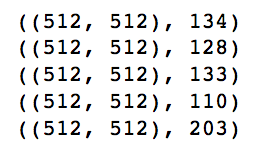
\includegraphics[width=0.3\textwidth]{dims.png}
\caption{\label{fig:Dimensions}Sample Dimensions of first five patients}
\end{figure}

Figure 1 illustrates the pixel sizes, 512 x 512 for each of the slices, and the last number represents the number of slices per patient, which is the first thing we will need to deal with.

This competition allows for external data. One possible source, which contains another 888 scans, is:

\href{https://luna16.grand-challenge.org/data/}{External Data}



\section{Techniques Overview}
What machine learning method(s) will you apply? Which packages?
How to handle issues such as class imbalance (for Vungle)? Size of the data for Kaggle? 
Kaggle teams: how do you preprocess your data?


Image Fusion using the Wavelet Transform


As was discussed in the ‘What Data?’ section, each observation comes in the form of many scans/slices. We are considering using a method called image fusion using the wavelet transform to compress many scans into one. This technique extracts the most salient/important features of each scan then merges them together. This will serve two purposes for us; 1) reduce the number of scans per observation, 2) it will normalize the number of scans per observation. For instance, if the observation has 300 scans 2mm apart we can merge every 10 scans using this technique, resulting in only 30 scans. If the observation has 150 scans 4mm apart we can merge every 5 scans, which also results in 30 scans. Each ‘merged’ scan in this case will cover 20mm.


The intuition behind this technique is that the cancerous nodule will only be evident in a few of the scans/slices covering some distance within the lungs. If we can qualitatively determine that the typical nodule is 20mm (for example) then we can merge the appropriate number of scans/slices to cover that distance. Then perhaps the nodule will be distinctly recognizable in one or two of the merged scans.
	There are some other contestants in this competition who have discussed simply averaging all of the scans to overcome the evident challenges with this input data. However, we this the above approach with yield more successful results.


The basis for our reasoning can be found in this paper: 
\href{http://old.vision.ece.ucsb.edu/publications/94ICIPWav.pdf}{Wavelet Transform}




3D Convolutional Neural Network

Once we have standardized the input data (scans) there will be ready for deep learning. Most image based classification uses convolutional neural networks. In this case we are not just dealing with one image per observation, but many. After researching some different methods to handle many images we have determined that it is similar to processing videos. Each scan/slice can be thought of as a frame in the video. Classification of videos using 3D convolutional neural networks area has been sufficiently studied. In fact, Keras supports fairly simple implementation of this method.


The basis for our reasoning can be found in this paper:

\href{http://www.cv-foundation.org/openaccess/content_iccv_2015/papers/Tran_Learning_Spatiotemporal_Features_ICCV_2015_paper.pdf}{3D Conv. Networks}




\section{Evaluation}
How will you verify your projects results and estimate whether you have solved the problem you have set out to address?

\section{Initial Results and EDA}


One transformation that may be of help is transforming pixel values into Hounsfield units. 


\section{Team responsibilities}
 
List the responsibilities of each person in the group in completing this part of the project assignment.

\end{document}